\section{Methods}\label{sec-methods} 

$\sequel$ can be broken down into four main steps: recruitment of reads to contigs; construction of the red-black positional de Bruijn graph; misassembly error prediction; and misassembly verification using optical mapping data.   
We explain each of these steps in detail in the following subsections. 


%\begin{figure}
        \begin{figure}[h!]
            \centering
              	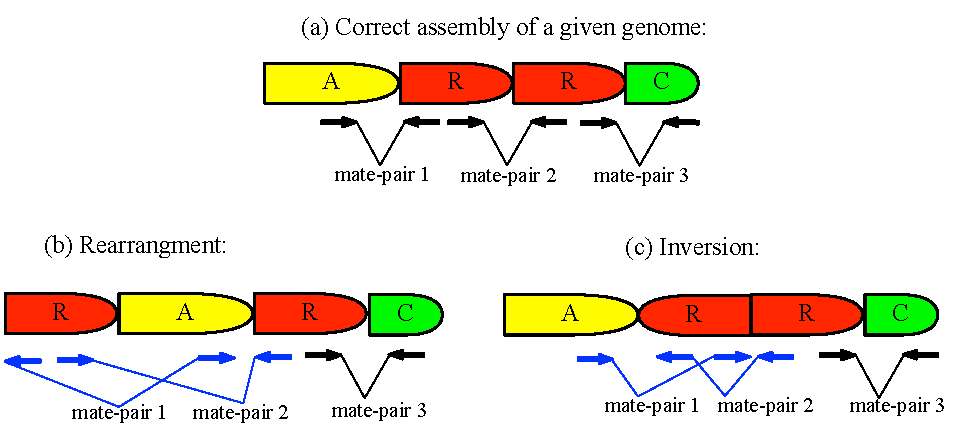
\includegraphics[width=0.6\textwidth]{./types_of_misassemblies_read_alignment.pdf}
                	\caption{An illustration of the systematic alterations that occur with rearrangements and inversions.  (a) Shows the proper read alignment where mate-pair reads have the correct orientation and distance from each other. A  rearrangement or	inversion will present itself by the orientation of the reads being incorrect, and/or the distance of the mate-pairs being significantly smaller or larger than the expected insert size. This is shown in (b) and (c), respectively.}
                	\label{fig:read_alignment_1}
        \end{figure}
      %\quad     
       	\begin{figure}[h!]
		\centering
                	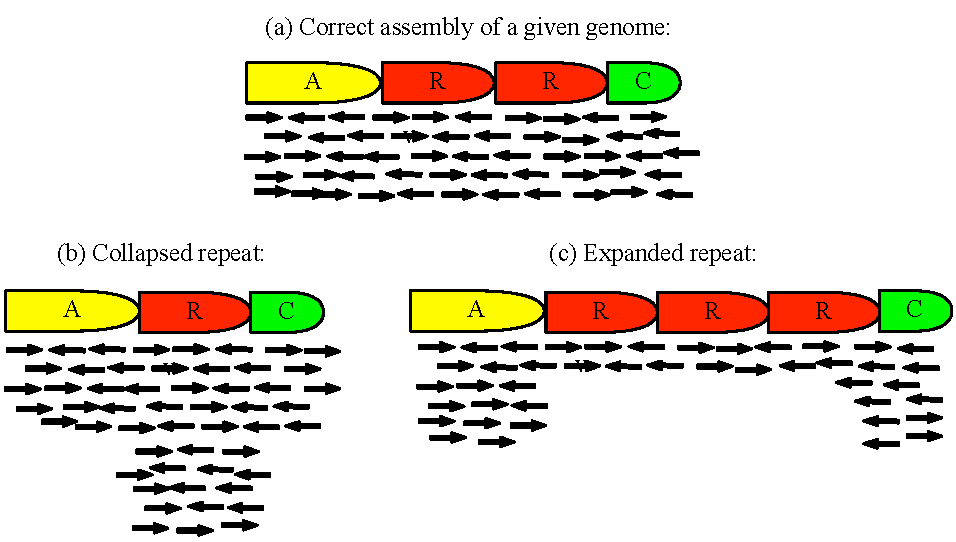
\includegraphics[width=0.6\textwidth]{./types_of_misassemblies_read_alignment_2.pdf}
       		\caption{An illustration of the systematic alterations that occur with collapsed or expanded repeats.  (a) Shows the proper read depth, which is uniform across the genome. A collapsed or expanded repeat will manifest as significantly lower or higher read depth; (b) shows a collapsed repeat, where the read depth being significantly greater than expected; and (c) shows a expanded repeat, where the observed read depth is significantly lower than expected.}
        		\label{fig:read_alignment_2}
        \end{figure}


\subsection{Recruitment of Reads and Threshold Calculation}  

$\sequel$ first aligns reads to contigs in order to identify regions that contain abnormal read alignments.  
Collapsed or expanded repeats will present as the read coverage being greater or lower than the expected genome coverage in the region that has been misassembled.  Similarly, inversion and rearrangement errors will present as the alignment of the mate-pairs being rearranged. Figures \ref{fig:read_alignment_1} and \ref{fig:read_alignment_2} illustrate these unconventional read alignments. More specifically, this step consists of aligning all the (paired-end) reads to all the contigs and then calculating three thresholds, $\Delta_L$, $\Delta_U$ and $\Gamma$.  The range $[\Delta_L, \Delta_U]$ defines the acceptable read depth, and $\Gamma$ defines the maximum allowable number of reads whose mate-pair aligns in an unconventional manner (e.g. inverted orientation). 
In order to calculate these thresholds, we consider all alignments of each read as opposed to just the best alignment of each read since misassembly errors frequently occur within repetitive regions where the reads will align to multiple locations.  
$\sequel$ performs this step using BWA (version 0.5.9) in paired-end mode with default parameters \cite{bwa}. % seems to be a specific detail, so past tense preserved, while elsewhere in this section keeping present tense to keep it more abstract
  Subsequently, after alignment, each contig is treated as a series of consecutive 200 bp regions.  These are sampled uniformly at random $\ell$ times, and the mean ($\mu_{d}$) and the standard deviation ($\sigma_d$) of the read depth and the mean ($\mu_{i}$) and the standard deviation ($\sigma_i$) of the number of alignments where an unconventional mate-pair orientation is witnessed are calculated from these sampled regions.   $\Delta_L$ is set to the maximum of $\{0, \mu_d - 3\sigma_d\}$, $\Delta_U$ is set to $\mu_d + 3\sigma_d$, and $\Gamma$ is set to $\mu_i + 3\sigma_i$.  The default for $\ell$ is $\frac{1}{20}$th of the contig length; this can be changed via an input parameter of $\sequel$.  

%Hence, any region where the read alignment has depth less than $\Delta_L$ or more than $\Delta_U$, or where the number of unconventional mate-pair alignments is greater than $\Gamma$ is considered abnormal.   


\subsection{Construction of the Red-Black Positional de Bruijn Graph} 


After threshold calculation, the red-black positional de Bruijn graph is constructed. For clarity, we begin by describing the {\em positional de Bruijn graph}, given by Ronen et al.~\cite{sequel}, and then define the red-black positional de Bruijn graph.  Whereas the edges in the traditional de Bruijn graph correspond to $k$-mers, the edges in the positional de Bruijn graph correspond to $k$-mers and their inferred positions on the contigs ({\em positional $k$-mers}).  Hence, the positional de Bruijn graph $G_{k, \Phi}$ is defined for a multiset of positional $k$-mers and parameter $\Phi$, and is constructed in a similar manner to the traditional de Bruijn graph using an A-Bruijn graph framework from \cite{PTT04}. Given a $k$-mer $s_k$, let $\prefix(s_k)$ be the first $k - 1$ nucleotides of $s_k$, and $\suffix(s_k)$ be the last $k - 1$ nucleotides of $s_k$.  Each positional $k$-mer $(s_k, p)$ in the input multiset corresponds to a directed edge in the graph between two positional $(k - 1)$-mers, $(\prefix(s_k), p)$ and $(\suffix(s_k), p + 1)$.  After all edges are formed, the graph undergoes a gluing operation. A pair of positional $(k - 1)$-mers, $(s_{k - 1}, p)$ and $(s_{k - 1}', p')$, are glued together into a single vertex if $s_{k - 1} = s_{k - 1}'$ and $p \in [p' - \Phi, p' + \Phi]$.  Two positional $(k - 1)$-mers are glued together if their sequences are the same and their positions are within $\Phi$ from each other. We refer to the {\em multiplicity} of a positional $(k - 1)$-mer $(s_{k - 1}, p)$ as the number of occurrences where $s_{k - 1}$ clustered at position $p$.  

$\sequel$ constructs the red-black positional de Bruijn graph from the alignment of the reads to the contigs. The red-black positional de Bruijn graph contains positional $k$-mers and is constructed in an identical way as the positional de Bruijn graph with the addition that each vertex ($(k - 1)$-mer) has an associated red or black color attributed to it that is defined using $\Delta_L$, $\Delta_U$ and $\Gamma$.  In addition to the multiplicity of each positional $(k - 1)$-mer, the number of positional $(k - 1)$-mers that originated from a read whose mate-pair did not align in the conventional direction is stored at each vertex.   When the multiplicity is less than $\Delta_L$ or greater than $\Delta_U$, or if the observed frequency of unconventional mate-pair orientation is greater than $\Gamma$, then the vertex is {\em red}; otherwise it is {\em black}.

\subsection{Misassembly Conjecture and Breakpoint Estimation}  

%Next, the red-black positional de Bruijn graph is used to detect misassembly errors and their breakpoints.  
A red-black positional de Bruijn graph is constructed for each contig, and misassembly errors in each contig are detected by searching for consecutive red vertices in the corresponding graph.  Depth-first search is used for the graph traversal. If there are greater than 50 consecutive red vertices then the contig is conjectured to be misassembled.  The breakpoint in the contig can be determined by recovering the position of the corresponding red vertices (e.g., the positional $(k - 1)$-mers).  The number of consecutive red vertices needed to consider it misassembled can be changed via a command line parameter in $\sequel$.  Our experiments were performed with the default (e.g. 50), which corresponds to a region in the contig that has length $\geq$ 50 bp.  After this stage of the algorithm, we take contigs having regions exceeding that threshold as a set of contigs that are conjectured to be misassembled and their transitions in and out of those regions as breakpoints.

%%%%%%%%%%%%%%%%%%%%%%%%%%%%
\subsection{Misassembly Verification} \label{dev}

% principles  
Lastly, we use optical mapping data to verify whether a contig that is conjectured to be misassembled indeed is.  
Verification is based on the expectation that, after {\em in silico} digestion, a correctly assembled contig has a sequence of fragment sizes that is similar to that in the optical map at the corresponding locus in the genome.  In other words, an {\em in silico} digested contig should align to some region of the optical map since both are derived from the same region in the genome.
Conversely, since misassembled contigs are not faithful reconstructions of any part of the genome, when {\em in silico} digested, their sequence of fragments will likewise not have a corresponding locus in the optical map to which it aligns.  
%However, there are exceptions to these principles.    

Optical maps contain measurement error at each fragment size so some criteria is needed to decide whether variation in fragment size of an {\em in silico} digested contig and that of an optical map at a particular locus is due to variation in the size of the physical fragments or a consequence of optical measurement error.  
Due to this ambiguity, and the necessary tolerances to ensure correctly assembled contigs align to the locus in the optical map, misassembled contigs may also align to loci in the optical map, which by coincidence have a fragment sequence similar to the contig within the threshold margin of error.  
While there are various sophisticated approaches to determining statistical significance of an alignment, such as by Sakar et al.~\cite{statsigORMalign}, we use a $ \chi^2 $ model discussed by Nagarajan et al.~\cite{soma} and take the cumulative density function $\le$ 0.85 as evidence of alignment, which we found to work well empirically.

% multiple optical maps
In addition, a misassembled contig only fails to align to the optical map if the enzyme recognition sequence, and thus the cleavage sites, exist in the contig in a manner that disrupts a good alignment (e.g. a misassembled contig with an inverted segment may still align if cleavage sites flank the inverted segment).
This implies that (a) some enzymes produce optical maps that have greater performance in identifying misassembly errors; and (b) alignment to the optical map is not as strong evidence for correct assembly as non-alignment to the optical map is for misassembly. 
This leads to the conclusion that an ensemble of optical maps (each made with a different enzyme) has a greater chance at revealing misassembly errors than a single optical map.  
Since acquiring three optical maps for one genome is reasonably accessible for many sequencing projects, the process of {\em in silico} digestion and alignment is repeated for three enzymes and the consensus of the alignment is taken over all of them, i.e., if two out of three times the contig did not align then it is deemed not to align (by the consensus).
A contig is deemed to be misassembled if it fails to align. The alignment is performed using Twin~\cite{wabi2014} (with default parameters) and then these results are filtered according to the $ \chi^2 $ model mentioned above.  
For our experiments, optical maps were simulated by {\em in silico} digesting reference genomes, adding normally distributed noise with a 150 bp standard deviation, and discarding fragments smaller than 700 bp.


     % 51 HP-xw6600-Xeon5450-SAS 8x3.0G 16Gb
     % 26 HP-Z210-XeonE3-1230 4x3.2G 8Gb
     % 26 HP-Z220-XeonE3-12230 4x3.3G 8Gb
     % 47 HP-z420-XeonE5-2650v2 8x2.6G 32Gb
